\chapter{Experimental Evaluation}

The focus of this chapter is:
\begin{enumerate}
\item the setup of the benchmark system,
\item the definition of the benchmarks, and
\item the results of the benchmarks
\end{enumerate}

\section{Benchmark System}
  \subsection{Hardware Setup}

The processor of the benchmark system is an Intel\textregistered~ Core\texttrademark~ i7-4771 CPU clocked at 3.50 GHz with 4 cores and hyperthreading enabled (which means 8 threads are available).
The benchmark system has a total amount of 16 GB of DDR3 RAM clocked at 1333 MHz available.

The root partition of the operating system is located on a ``Samsung SSD 840'' solid state drive (SSD).
It is installed on an ext4 filesystem.

The \texttt{hdparm} program gives an idea of how much throughput the SSD can handle. The results are listed in the table \ref{eval-ssd} on page \pageref{eval-ssd}.

\begin{table}[h]
\centering
\caption{Read performance of the benchmark SSD}
\label{eval-ssd}
\begin{tabular}{lrrr}
\textbf{}                   & \textbf{data read} & \textbf{time} & \textbf{result} \\ \hline
Timing cached reads         & $28536$ MB         & $1.99$ s      & $14316.64$ MB/s \\
Timing buffered disk reads: & $1608$ MB          & $3.00$ s      & $535.47$ MB/s   \\ \hline
\end{tabular}
\end{table}

All benchmarks are performend on the SSD.

  \subsection{Software Setup}

The operating system Fedora 27 is used for executing the benchmarks.
Elektra version 0.8.21 at the git commit \texttt{dfa9bb8}\footnote{The full commit hash is dfa9bb89ada39996cac5c1abd21481e1e2181ad9.} is installed on the system.

The most important program versions are listed below:

\begin{itemize}
  \item clang version 5.0.1 (tags/RELEASE\_501/final)
  \item Botan version 1.10.17-1.fc27
  \item OpenSSL version 1.1.0g-1.fc27
  \item libgcrypt version 1.8.2-1.fc27
  \item GnuPG version 2.2.4-1.fc27
\end{itemize}

Listing \ref{eval-compile} on page \pageref{eval-compile} shows how \elektra ~ is compiled on the benchmark system.

\begin{code}[label=eval-compile,language=bash,caption={Elektra compile options for the benchmarks}]
mkdir build && cd build
cmake -GNinja \
    -DBUILD_STATIC=OFF \
    -DCMAKE_C_COMPILER=clang \
    -DCMAKE_CXX_COMPILER=clang++ \
    -DBUILD_DOCUMENTATION=OFF \
    -DCMAKE_INSTALL_PREFIX=/usr \
    ..
ninja install
\end{code}

  \subsection{Time Measurement}

The runtime of a benchmark is measured using the system time, which is returned by the system function \texttt{gettimeofday ()}.
The time measurement is abstracted in a class called \texttt{Timer}.
Listing \ref{eval-time} on page \pageref{eval-time} demonstrates how a benchmark is written.

\begin{code}[label=eval-time,language=C,caption={Time measurement for the benchmarks}]
void do_benchmark ()
{
  Timer t();

  // begin of measurement
  t.start ();

  action_to_be_measured ();

  // end of measurement
  t.end ();
}
\end{code}

  \subsection{Statistical Method}

Every benchmark run is repeated 11 times.
For the sorted set of results $\{r_{1},...,r_{11} | r_n \leq r_{n+1}\}$ the median is given as $\tilde{x}=r_6$.

The median is chosen as measurement result because of its robustness against outliers.
When we speak of the result of a benchmark, we always refer to the median $\tilde{x}$ of the 11 benchmarks runs.

\section{Benchmark 1 -- Runtime Comparison}
\label{eval-bench-one}

This benchmark examines the runtime performance of the \crypto ~.
The benchmark compares the duration of the \texttt{kdb set} and \texttt{kdb get} methods:

\begin{enumerate}
\item without the \crypto ,
\item with the \fcrypt ,
\item with the \texttt{crypto\_openssl} plugin variant,
\item the \texttt{crypto\_gcrypt} plugin variant, and 
\item the \texttt{crypto\_botan} plugin variant.
\end{enumerate}

For each benchmark variant an Elektra backend is set up.
For every backend a configuration setting with a preset size is generated.
First the duration of the \texttt{kdb set} method of Elektra is being measured, which represents the performance of the encryption process.
Then the duration of the \texttt{kdb get} method of Elektra is being measured, which represents the performance of the decryption process.
The benchmark is repeated with configuration setting sizes, that ranges from $1$ to $1000$.

For better reproducibility we provide a script, that executes the benchmark as we do in this thesis.
The script is available at Github\footnote{\url{https://github.com/petermax2/libelektra-crypto-benchmarks/blob/master/scripts/start-crypto-comparison.sh}}.

  \subsection{Benchmark Code}

The source code of the benchmark is distributed with Elektra, and it is located at\\
\texttt{libs/tools/benchmarks/benchmark\_crypto\_comparison.cpp}.

Listing \ref{eval-1-code} on page \pageref{eval-1-code} is an excerpt of the benchmark code.
The listing gives an idea about how the measurement is accomplished.
The listing has been slightly modified to improve readability, but the execution flow has not been altered.

\begin{code}[label=eval-1-code,language=C,caption={Excerpt of Benchmark 1}]
static Timer t (plugin_variant_names[VARIANT]);
Key mp = mountBackend<VARIANT> (iteration);
{
  KDB kdb;
  KeySet ks;

  kdb.get (ks, mp);
  // n = size of the configuration setting
  for (int i = 0; i < n; ++i)
  {
    ks.append (Key (mp.getName () + "/k" + std::to_string (i),
      KEY_VALUE, "value",
      KEY_META, "crypto/encrypt", "1",
      KEY_END));
  }

  t.start (); // start of the measurement
  kdb.set (ks, mp);
  t.stop (); // end of the measurement

  kdb.close ();
}
std::cout << t;
\end{code}

  \subsection{Results of the Runtime Comparison}
  \label{eval-section-runtime-results}

The runtime results of all benchmark runs are listed in chapter \ref{chapter-benchmark-results} on page \pageref{chapter-benchmark-results}.
The results are also published at Github\footnote{\url{https://github.com/petermax2/libelektra-crypto-benchmarks/tree/master/results}}.
Figure \ref{eval-runtime-comp-set} on page \pageref{eval-runtime-comp-set} compares the benchmark results of all tested variants for the \texttt{kdb set} method.
Figure \ref{eval-runtime-comp-get} on page \pageref{eval-runtime-comp-get} provides a comparison of the benchmark results of all tested variants for the \texttt{kdb get} method.

\begin{figure}[h]
\center
\caption{Runtime comparison of \texttt{kdb set}}
\label{eval-runtime-comp-set}
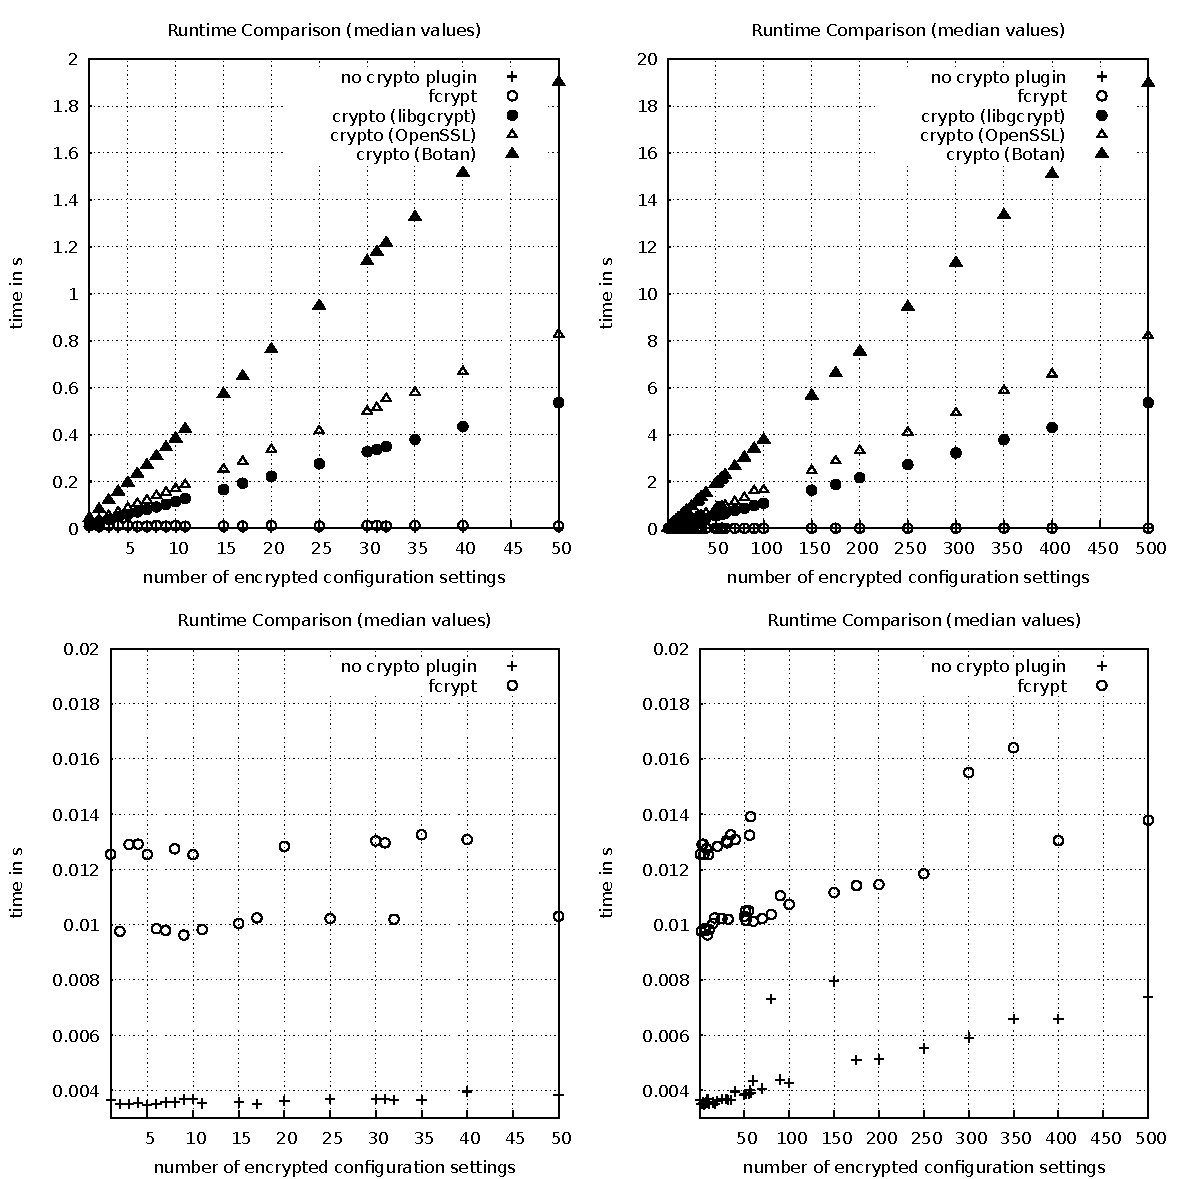
\includegraphics[width=\columnwidth]{plots/comp_median_set.pdf}
\end{figure}

\begin{figure}[h]
\center
\caption{Runtime comparison of \texttt{kdb get}}
\label{eval-runtime-comp-get}
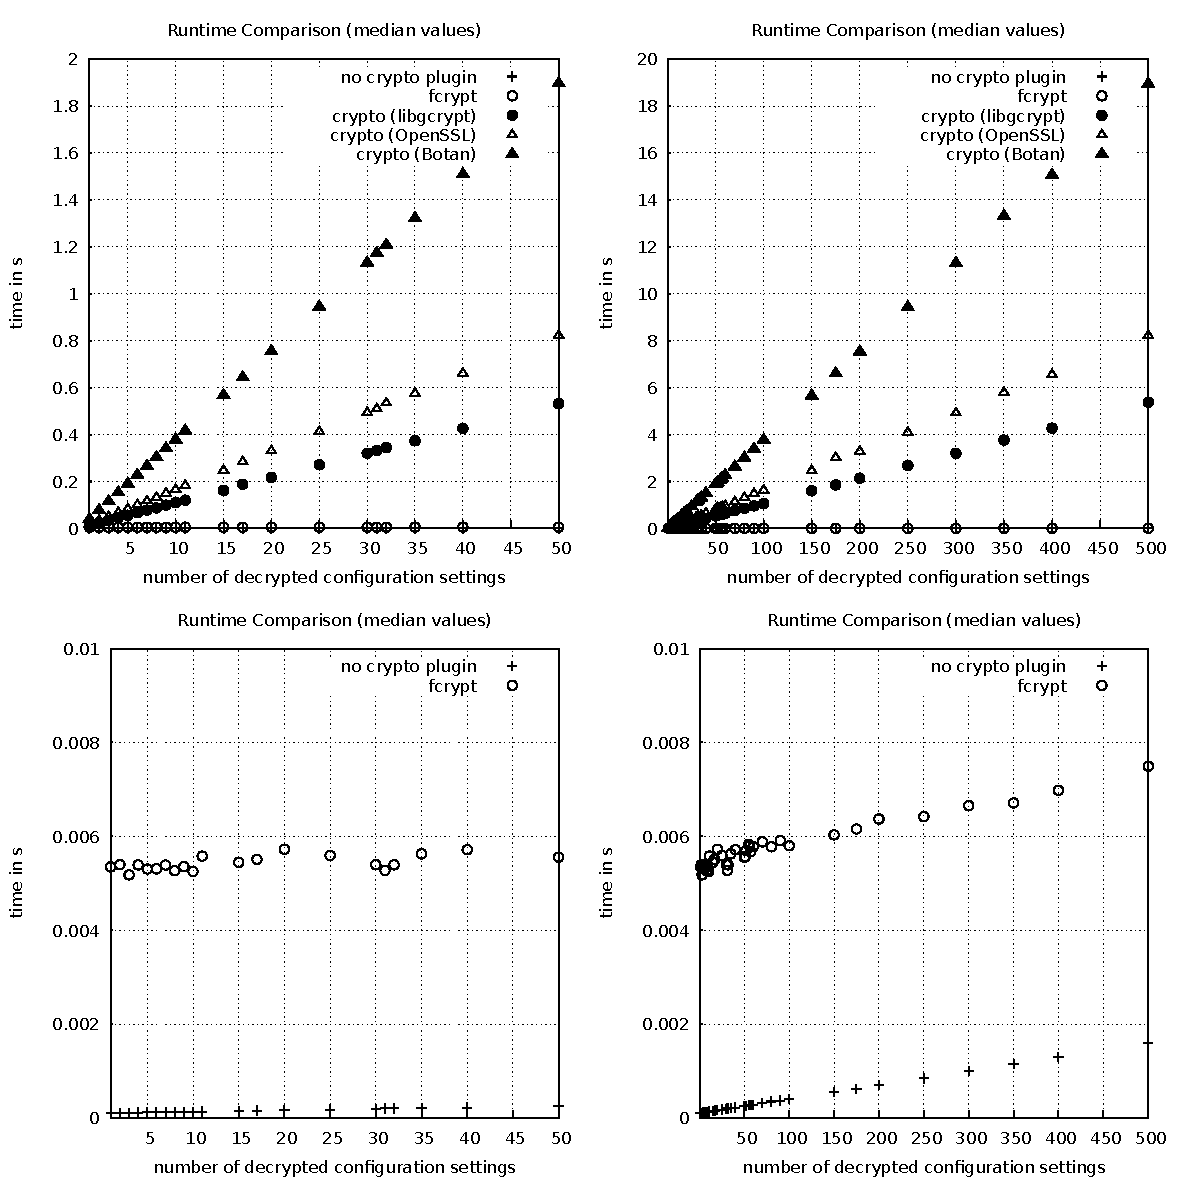
\includegraphics[width=\columnwidth]{plots/comp_median_get.pdf}
\end{figure}

As we can see from the benchmark results, the runtime behavior has a tendency to increase linearly with the number of encrypted/decrypted configuration values.

The boxplot in figure \ref{eval-boxplot-set} on page \pageref{eval-boxplot-set} shows that the benchmark results for the \texttt{kdb set} are stable.
There are no noteworthy outliers.
Figure \ref{eval-boxplot-get} on page \pageref{eval-boxplot-get} reveals analogous insights for the \texttt{kdb get} method.

\begin{figure}[h]
\center
\caption{Boxplots of the \texttt{kdb set} runtime with $n = 500$ configuration settings}
\label{eval-boxplot-set}
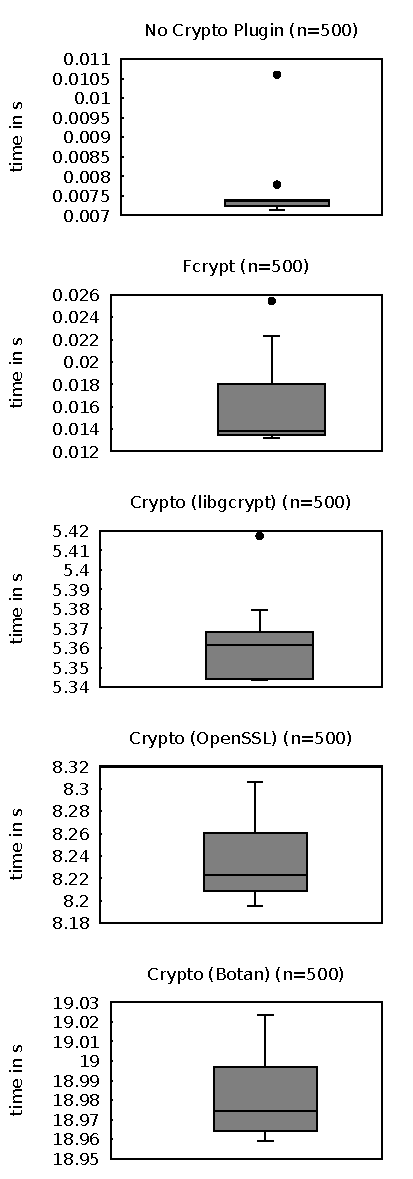
\includegraphics{plots/boxplot_500_set.pdf}
\end{figure}

\begin{figure}[h]
\center
\caption{Boxplots of the \texttt{kdb get} runtime with $n = 500$ configuration settings}
\label{eval-boxplot-get}
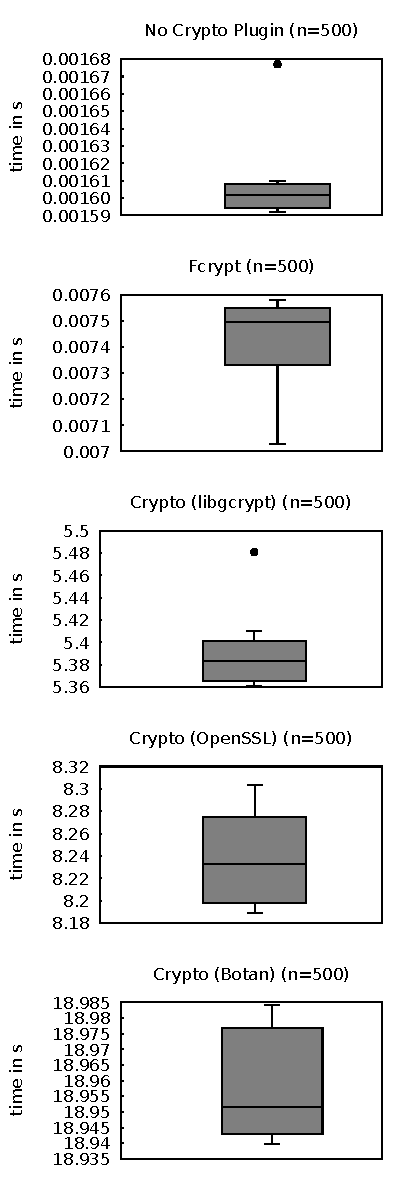
\includegraphics{plots/boxplot_500_get.pdf}
\end{figure}


\section{Benchmark 2 -- Memory Analysis}
\label{eval-bench-two}

This benchmark examines the memory allocations of the \crypto ~.
The benchmark code is the same as for Benchmark 1 (see Section \ref{eval-bench-one} on page \pageref{eval-bench-one}).

	\subsection{Massif Analysis}

The benchmark code of benchmark 1 is analysed using Valgrind's Massif tool.
Massif-Visualizer is used to produce a visualization of the data, that is collected by Massif.

The benchmark is started with the following configuration setting sizes $n$:

\begin{itemize}
\item 10
\item 100
\item 200
\end{itemize}

	\subsection{Results of the Memory Analysis}

The results of the memory analysis  are published on Github
\footnote{\url{https://github.com/petermax2/libelektra-crypto-benchmarks/tree/master/massif}}.

Figures
\begin{itemize}
\item \ref{eval-massif-010} on page \pageref{eval-massif-010},
\item \ref{eval-massif-100} on page \pageref{eval-massif-100}, and
\item \ref{eval-massif-200} on page \pageref{eval-massif-200}
\end{itemize}
show the visualizations, that have been produced by Massif-Visualizer.

\begin{sidewaysfigure}
\center
\caption{Result Of The Memory Analysis with $n = 10$ configuration settings}
\label{eval-massif-010}
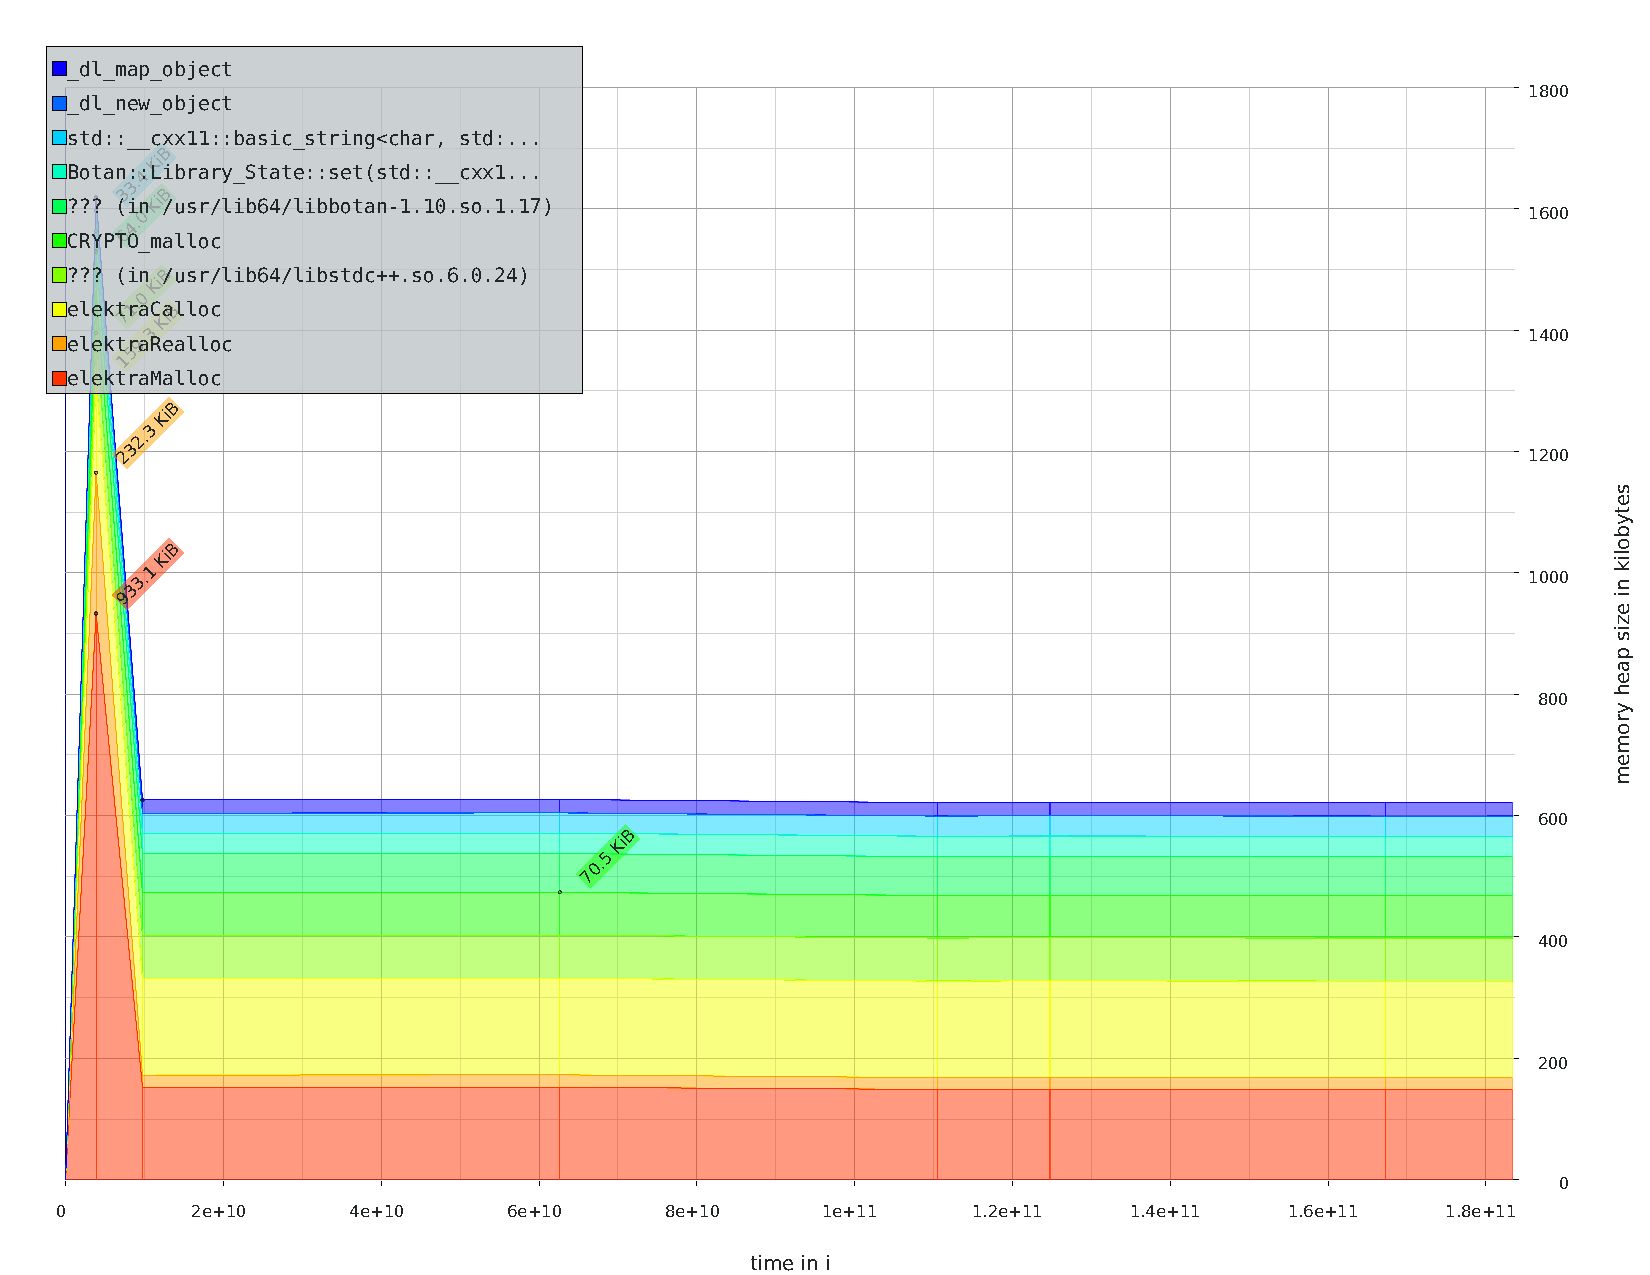
\includegraphics[width=\columnwidth]{plots/massif_010.pdf}
\end{sidewaysfigure}

\begin{sidewaysfigure}
\center
\caption{Result Of The Memory Analysis with $n = 100$ configuration settings}
\label{eval-massif-100}
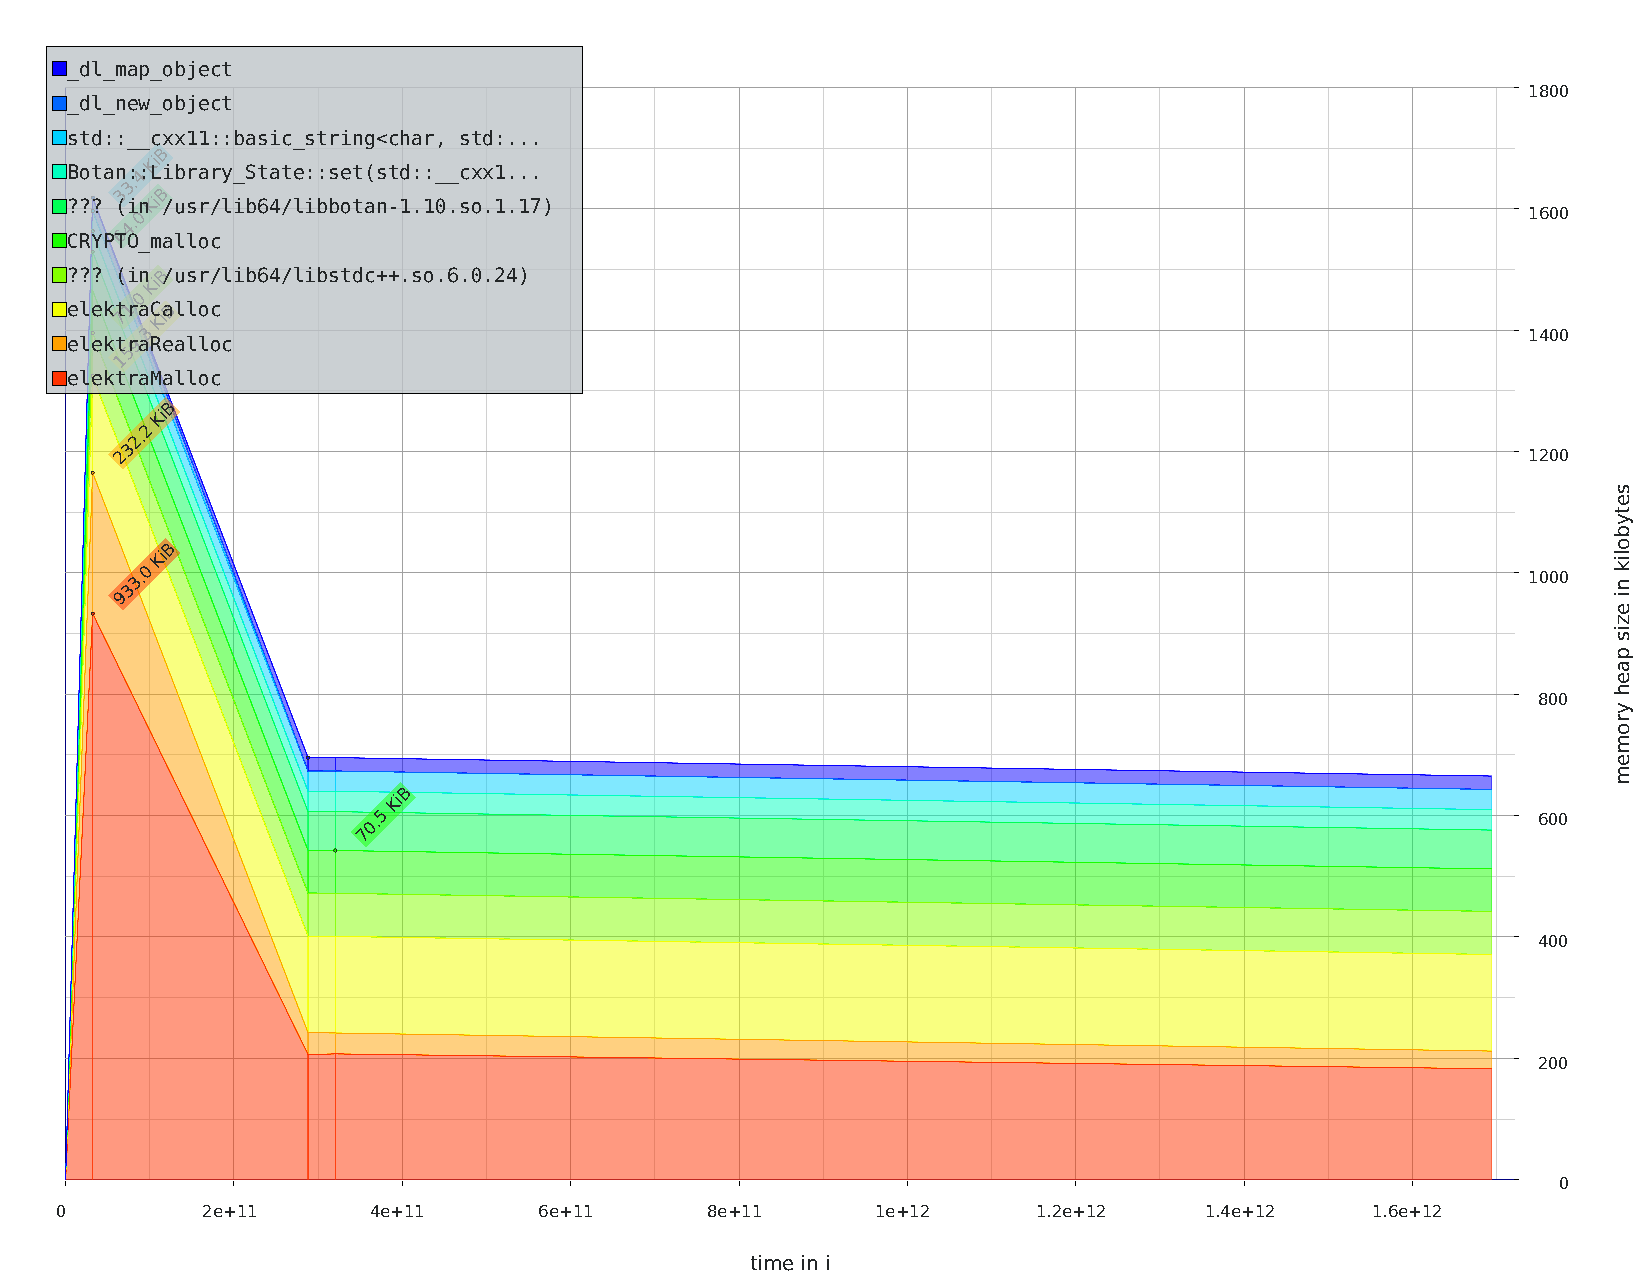
\includegraphics[width=\columnwidth]{plots/massif_100.pdf}
\end{sidewaysfigure}

\begin{sidewaysfigure}
\center
\caption{Result Of The Memory Analysis with $n = 200$ configuration settings}
\label{eval-massif-200}
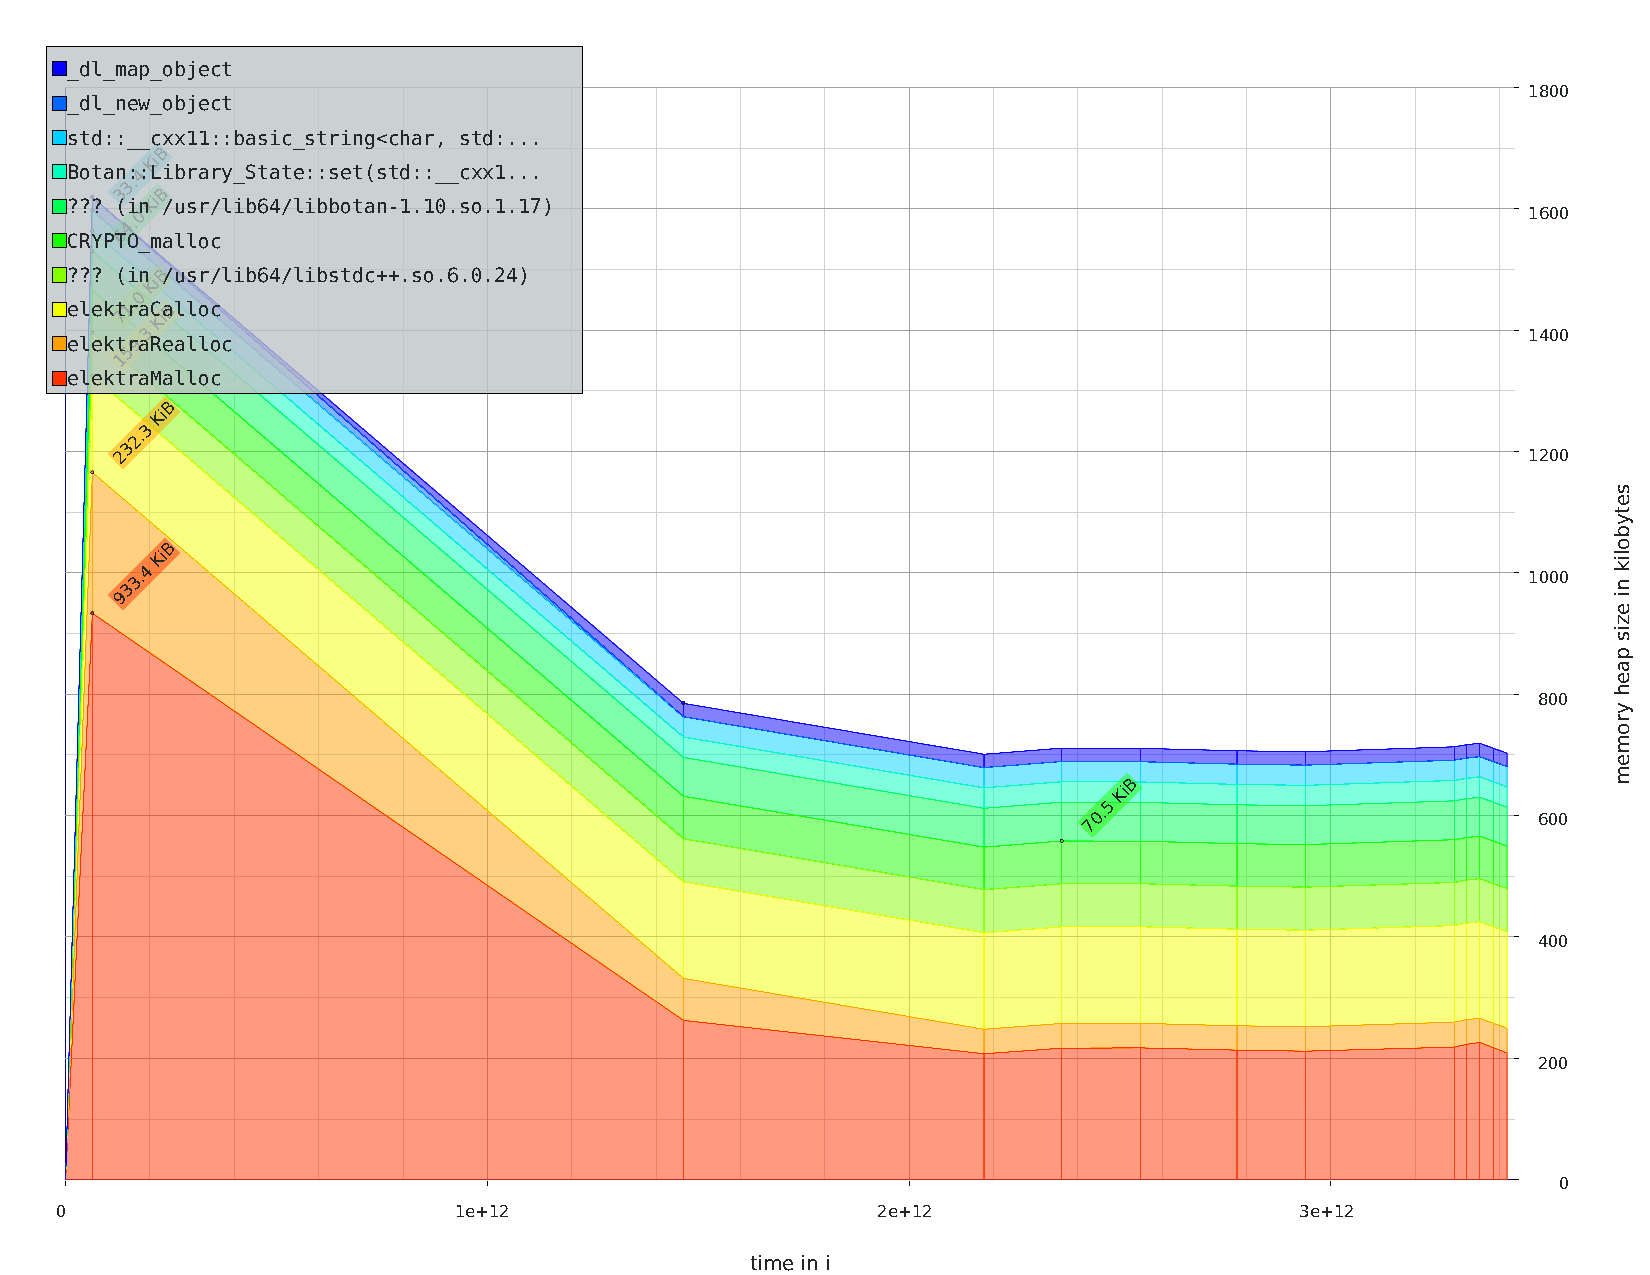
\includegraphics[width=\columnwidth]{plots/massif_200.pdf}
\end{sidewaysfigure}

